\documentclass[12pt]{article}

\pagestyle{empty}
\setcounter{secnumdepth}{2}
%----------------------------------------------------------------------------------------
%   Defines
%----------------------------------------------------------------------------------------

%----------------------------------------------------------------------------------------
%   Packages and configurations
%----------------------------------------------------------------------------------------
\usepackage[dutch]{babel}
\usepackage{hyperref} %Allow for references
\usepackage{lastpage}
\usepackage{fancyheadings}
\hypersetup{
colorlinks,
citecolor=black,
filecolor=black,
linkcolor=black,
urlcolor=black
} %Set up hyperlink colours.
\newcommand{\sectionbreak}{\clearpage} % Should start every section on its own page
\usepackage{geometry} % Required to change the page size to A4
\geometry{a4paper} % Set the page size to be A4 as opposed to the default US Letter
\usepackage{chngpage}
\usepackage{appendix}
%REMOVE IF HEADER/FOOTER BROKEN
\usepackage{fancyhdr} % Required for custom headers
\usepackage{extramarks} % Required for headers and footers
\usepackage{lastpage} % Required to determine the last page for the footer
%-----------------1
\topmargin=0cm
\oddsidemargin=0cm
\textheight=22.0cm
\textwidth=16cm
\parindent=0cm
\parskip=0.15cm
\topskip=0truecm
\raggedbottom
\abovedisplayskip=3mm
\belowdisplayskip=3mm
\abovedisplayshortskip=0mm
\belowdisplayshortskip=2mm
\normalbaselineskip=12pt
\normalbaselines
\usepackage{listings}
\usepackage[svgnames,table,xcdraw]{xcolor}
\lstset { 
language=C,
frame=single,
escapeinside={\%*}{*)}, 
breaklines=true,  
backgroundcolor=\color{black!5},
basicstyle=\footnotesize,
commentstyle=\color{mygreen},
numberstyle=\tiny\color{mygray},
rulecolor=\color{black},
keywordstyle=\color{blue},
}

\definecolor{mygreen}{rgb}{0,0.6,0}
\definecolor{mygray}{rgb}{0.5,0.5,0.5}
\definecolor{mymauve}{rgb}{0.58,0,0.82}
\usepackage{wasysym}
\pagestyle{fancy}
\lhead{Jim \textsc{van Abkoude} \& Julian G. \textsc{West}} % Top left header
\rhead{Opdrachten week \weeknumber} % Top center header
\lfoot{
\includegraphics[height=0.8cm]{avans}} % Bottom left footer
\cfoot{} % Bottom center footer
\rfoot{Pagina\ \thepage} % Bottom right footer
\renewcommand\headrulewidth{0.4pt} % Size of the header rule
\renewcommand\footrulewidth{0.4pt} % Size of the footer rule
\usepackage{graphicx} % Required for including pictures

\usepackage{float} % Allows putting an [H] in \begin{figure} to specify the exact location of the figure
\usepackage{wrapfig} % Allows in-line images such as the example fish picture
\usepackage{lipsum} % Used for inserting dummy 'Lorem ipsum' text into the template
\usepackage{pdfpages}
\usepackage[font={footnotesize}]{caption}
\graphicspath{{imgs/}}
\setlength\parindent{0pt} % Removes all indentation from paragraphs
%\usepackage{showframe}
\newcommand*{\SignatureAndDate}[1]{%
    \par\noindent\makebox[2.5in]{\hrulefill} \hfill\makebox[2.0in]{\hrulefill}%
    \par\noindent\makebox[2.5in][l]{#1}      \hfill\makebox[2.0in][l]{Date}%
}%Signature package

%----------------------------------------------------------------------------------------
%   Document start
%----------------------------------------------------------------------------------------
\begin{document}
\newcommand{\weeknumber}{4}

\begin{titlepage}
\pagenumbering{Roman}
\newcommand{\HRule}{\rule{\linewidth}{0.5mm}} % Defines a new command for the horizontal lines, change thickness here

\center % Center everything on the page


\includegraphics[height=3cm]{avans}\\% Include a department/university logo - this will require the graphicx package
\textsc{\Large Avans Hogeschool Breda}\\[0.5cm] % Major heading such as course name
\textsc{\large Intelligente wireless sensornetwerken}\\[0.5cm] % Minor heading such as course title
\HRule \\[0.4cm]
{ \huge \bfseries Opdrachten week \weeknumber}\\[0.4cm] % Title of your document
\HRule \\[1.5cm]

\begin{minipage}{0.4\textwidth}
\begin{flushleft} \large
\emph{Auteurs:}\\
Jim \textsc{van Abkoude} \\
Julian \textsc{West} \\
\end{flushleft}
\end{minipage}
~
\begin{minipage}{0.4\textwidth}
\begin{flushright} \large
\emph{Docenten:} \\
Diederich \textsc{Kroeske} \\ % Supervisor's Name
Andries \textsc{van Dongen} \\ % Supervisor's Name
\end{flushright}
\end{minipage}\\[4cm]

{\large \today}\\[3cm] % Date, change the \today to a set date if you want to be precise

Versie: 0.1.0

\vfill % Fill the rest of the page with whitespace

\end{titlepage}

\clearpage

\pagenumbering{arabic}
\section{Setup}

Voor deze opdracht willen wij een remote REST server hebben om data mee op te slaan. Deze zal via Node.js ontvangen gegevens in een database opslaan. De structuur van de database is niet belangrijk, we zullen de algemene data opslaan in de velden ID (van de meeting, uniek, van Node.js script), Time (timestamp, van Node.js), Source(welk device, van zender), Type (van de meting, van zender), values (kan alles zijn, kunnen meerdere velden worden, van zender). \\
De devices die we hebben stellen in met de opgelegde structuur. Allen in API mode, 1 coördinator, 2 routers en 2 end devices. De coördinator krijgt als bonus de ethernet shield, zodat deze de ontvangen data doorsluizen naar de REST server. De opstelling wordt weergegeven in figuur~\ref{fig:setup1}.\\
Na veel gedoe en werk is een soort-van REST server opgezet in Node.js die via een HTTP POST actie met JSON als inhoud, deze data opslaan in een MySQL database. Deze JSON request moet opgebouwd zoals in het voorbeeld hieronder. Het "id" veld kan worden gegenereerd, en hoeft niet ingevoerd te worden. Als een "id" al voorkomt in de database, zal de post niet succesvol zijn. Een ietwat aangepast, maar nog functionele, versie van de Node.js code staat in bijlage 1.\\
Figuren~\ref{fig:rest_test1} tot~\ref{fig:rest_test3} laten de werking van de REST server zien. \\
Deze server had niet kunnen werken zonder de input en samenwerking van Joris, Guus en Jelle. Daarvoor heel erg bedankt. Als teken van dank helpen we elkaar om dit moment. 
\begin{lstlisting}
{
	"id": x,
	"meetopstellingen": x,
	"timestamp": "jjjj-mm-dd hh:MM:ss",
	"waarde": "string"
}
\end{lstlisting}
\clearpage
\begin{figure}
\begin{center}
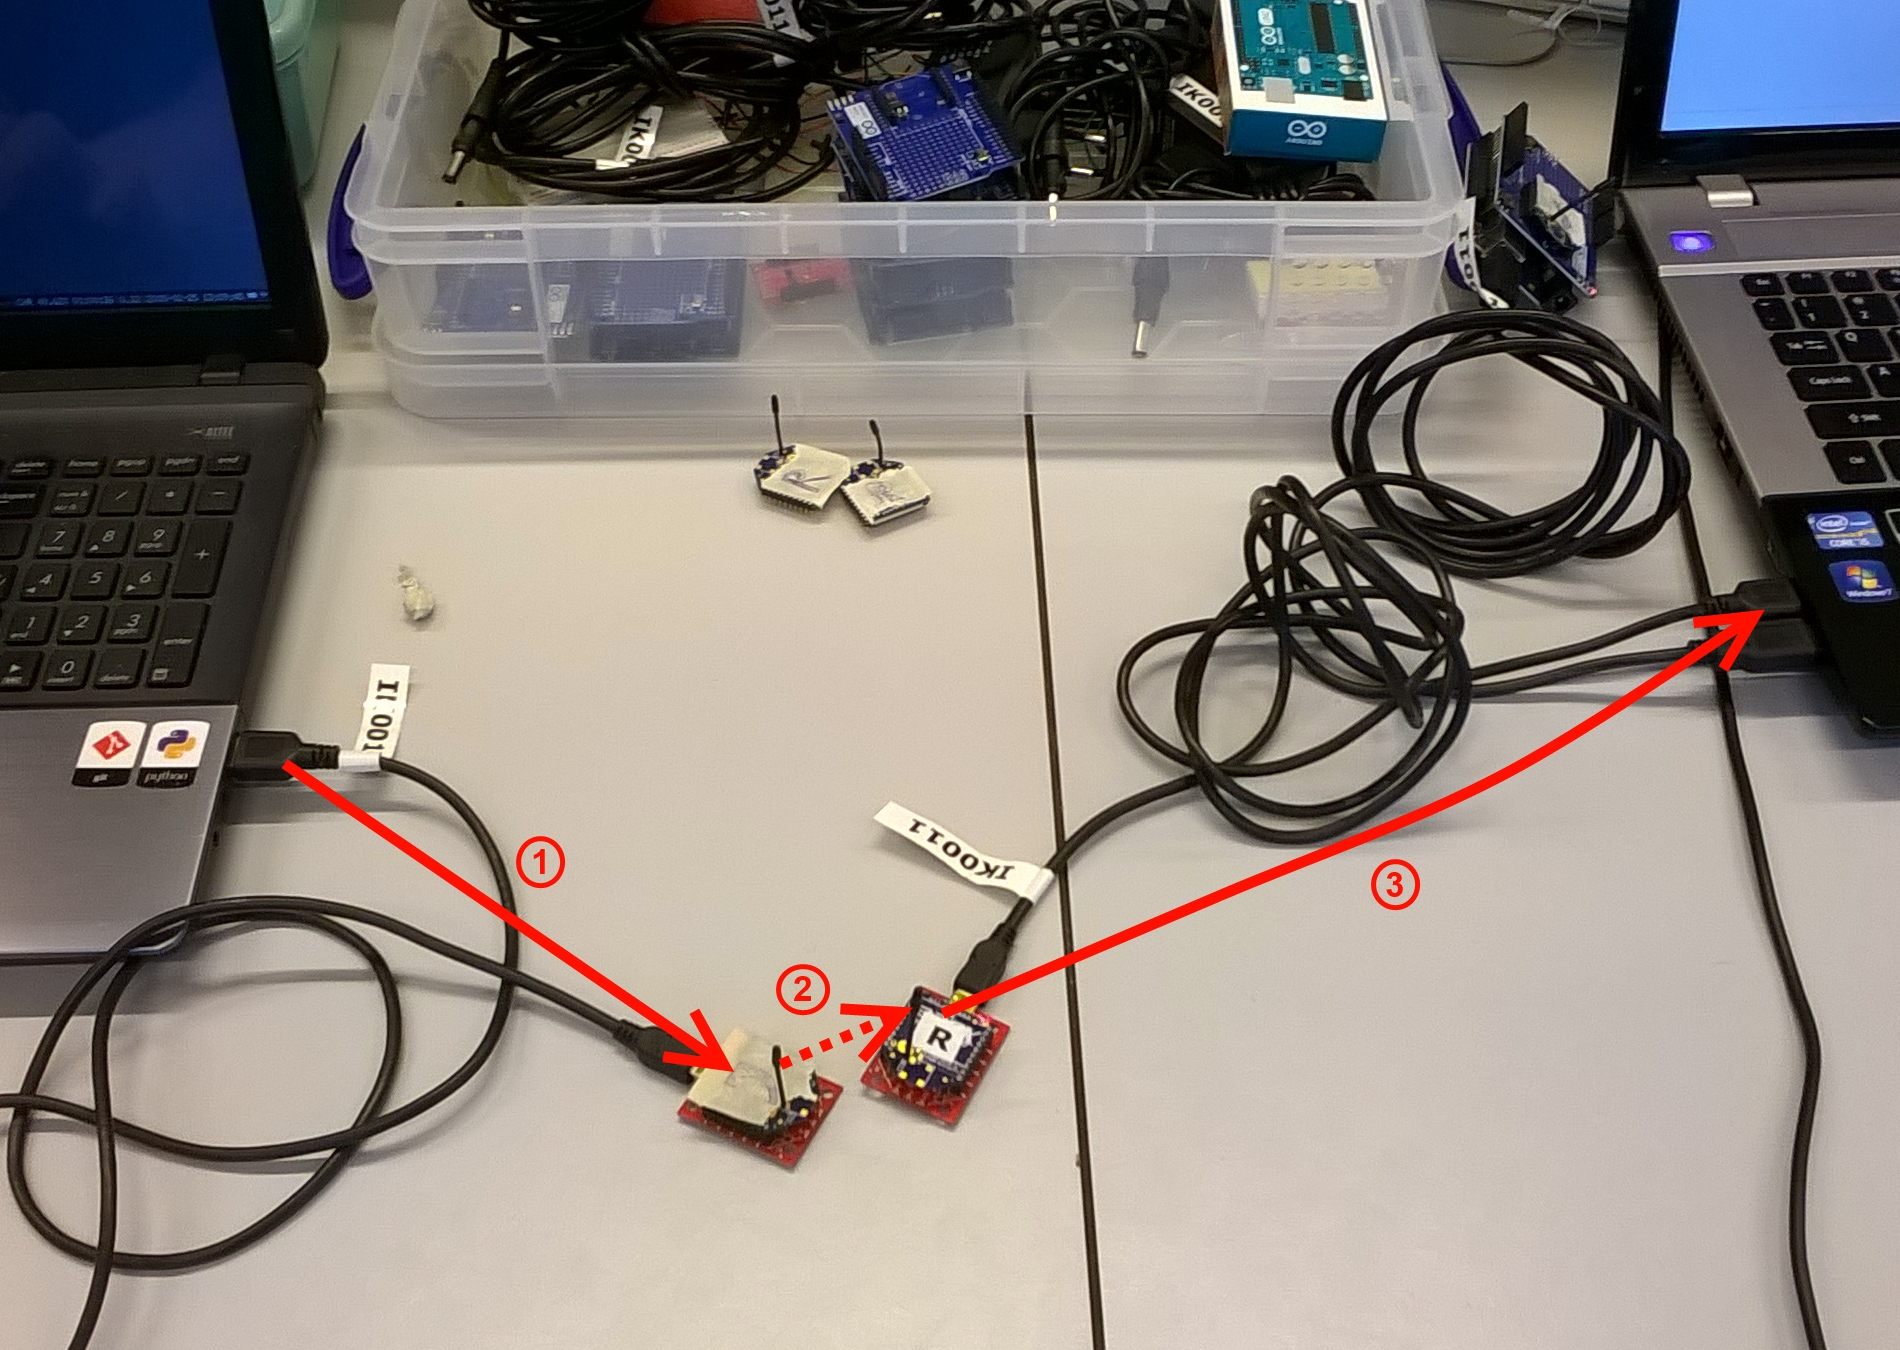
\includegraphics[scale=.4]{Test_Setup_1.jpg}
\caption{Initiële opstelling apparaten}
\label{fig:setup1}
\end{center}
\end{figure}
\begin{figure}
\begin{center}
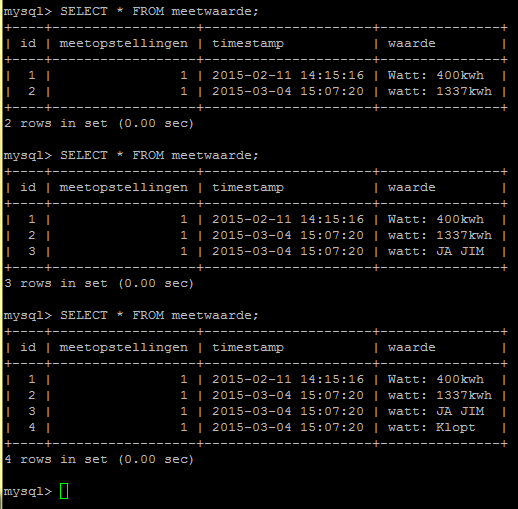
\includegraphics[scale=1]{Rest_test_1.png}
\caption{MySQL resultaten na elke (succesvolle) insert}
\label{fig:rest_test1}
\end{center}
\end{figure}
\begin{figure}
\begin{center}
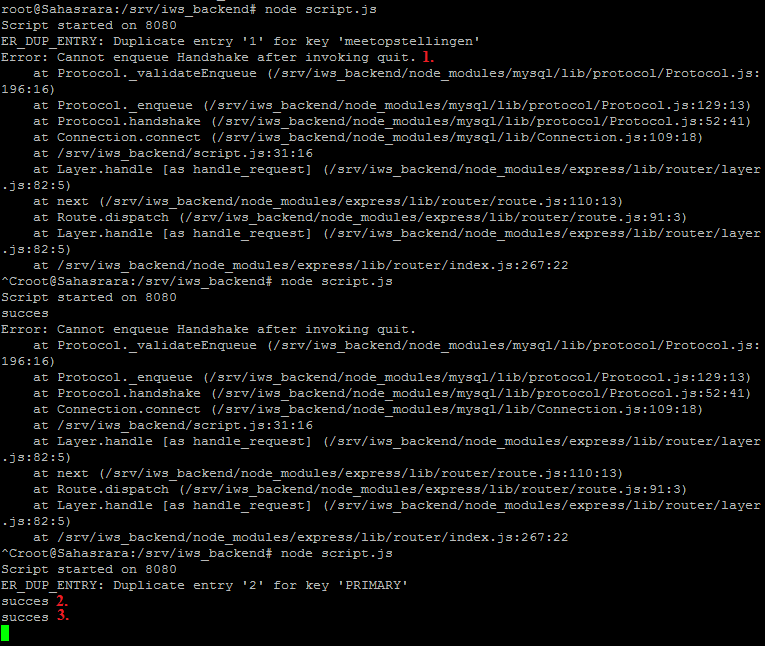
\includegraphics[scale=.9]{Rest_test_2.PNG}
\caption{Node output met 1. foutieve input 2. succesvolle input 3. succesvolle input}
\label{fig:rest_test2}
\end{center}
\end{figure}
\begin{figure}
\begin{center}
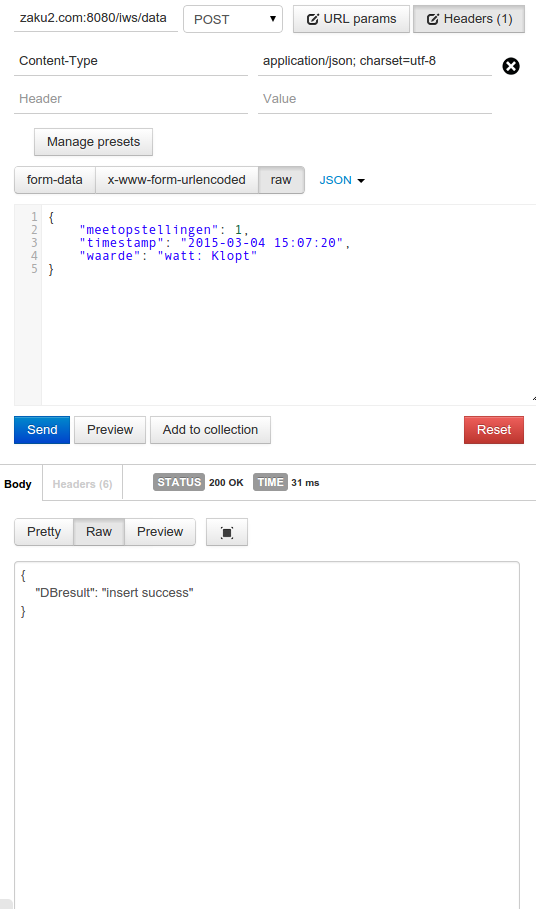
\includegraphics[scale=.6]{Rest_test_3.png}
\caption{POST debug tool, post zonder ID, return is succes}
\label{fig:rest_test3}
\end{center}
\end{figure}
\clearpage
\section{Opdrachten}

\subsection*{1a}
Voor de setup die we hebben gemaakt, zie hoofdstuk 1. De PANID die wij hebben gekozen is 4016.
\subsection*{1b}

\begin{figure}[h]
\begin{center}
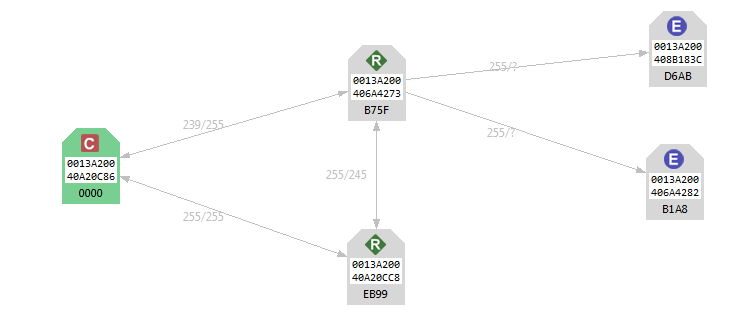
\includegraphics[scale=.8]{API_network.png}
\caption{Het netwerk zoals weergegeven in XCTU met 64- en 16-bit adres}
\label{fig:api_net}
\end{center}
\end{figure}
\begin{table}[h]
\begin{center}
\begin{tabular}{lll}
\rowcolor[HTML]{656565} 
\textbf{Type} 	  & \textbf{64-bit adres: 0013A200...} & \textbf{16-bit adres}\\
Co\"{o}rdinator   & ...40A20C86       &  0000	\\
Router            & ...406A4273       &  B75F  \\
Router A      	  & ...40A20CC8       &  EB99  \\
End device B      	  & ...408B183C       & D6AB   \\
End device C      	  & ...406A4282       &	B1A8	\\               
\end{tabular}
\end{center}
\caption{Tabel van XBee modules en hun (lage) 64-bit adres}
\label{tab:info1}
\end{table}
\clearpage

\section{Bijlage}
\subsection*{Bijlage 1}
Beknopte versie van de Node.js code voor pseudo REST server om functionaliteit te testen. Commentaar is weggelaten.
\begin{lstlisting}
var mysql      = require('mysql');
var connection = mysql.createConnection({
  host     : 'localhost',
  user     : 'us',
  password : 'controller',
  database : 'iws_week4'
  });

var express    = require('express');
var app        = express();  
var bodyParser = require('body-parser');
var port = process.env.PORT || 8080;

app.use(bodyParser.urlencoded({ extended: true }));
app.use(bodyParser.json()); 
var router = express.Router(); 

connection.connect();

router.route('/data').post(function(req, res) {
  var post= req.body;
  connection.query('INSERT INTO meetwaarde SET ?', post, function(error){
   if(error){
     console.log(error.message);
     res.json({ DBresult: 'insert failure' });
     }else{
       console.log('succes');
       res.json({ DBresult: 'insert success' });
     }
     });
  
  });

app.use('/iws', router);

app.listen(port);
console.log('Script started on ' + port);
\end{lstlisting}
\end{document}
